\begin{figure}[H]
  \centering
  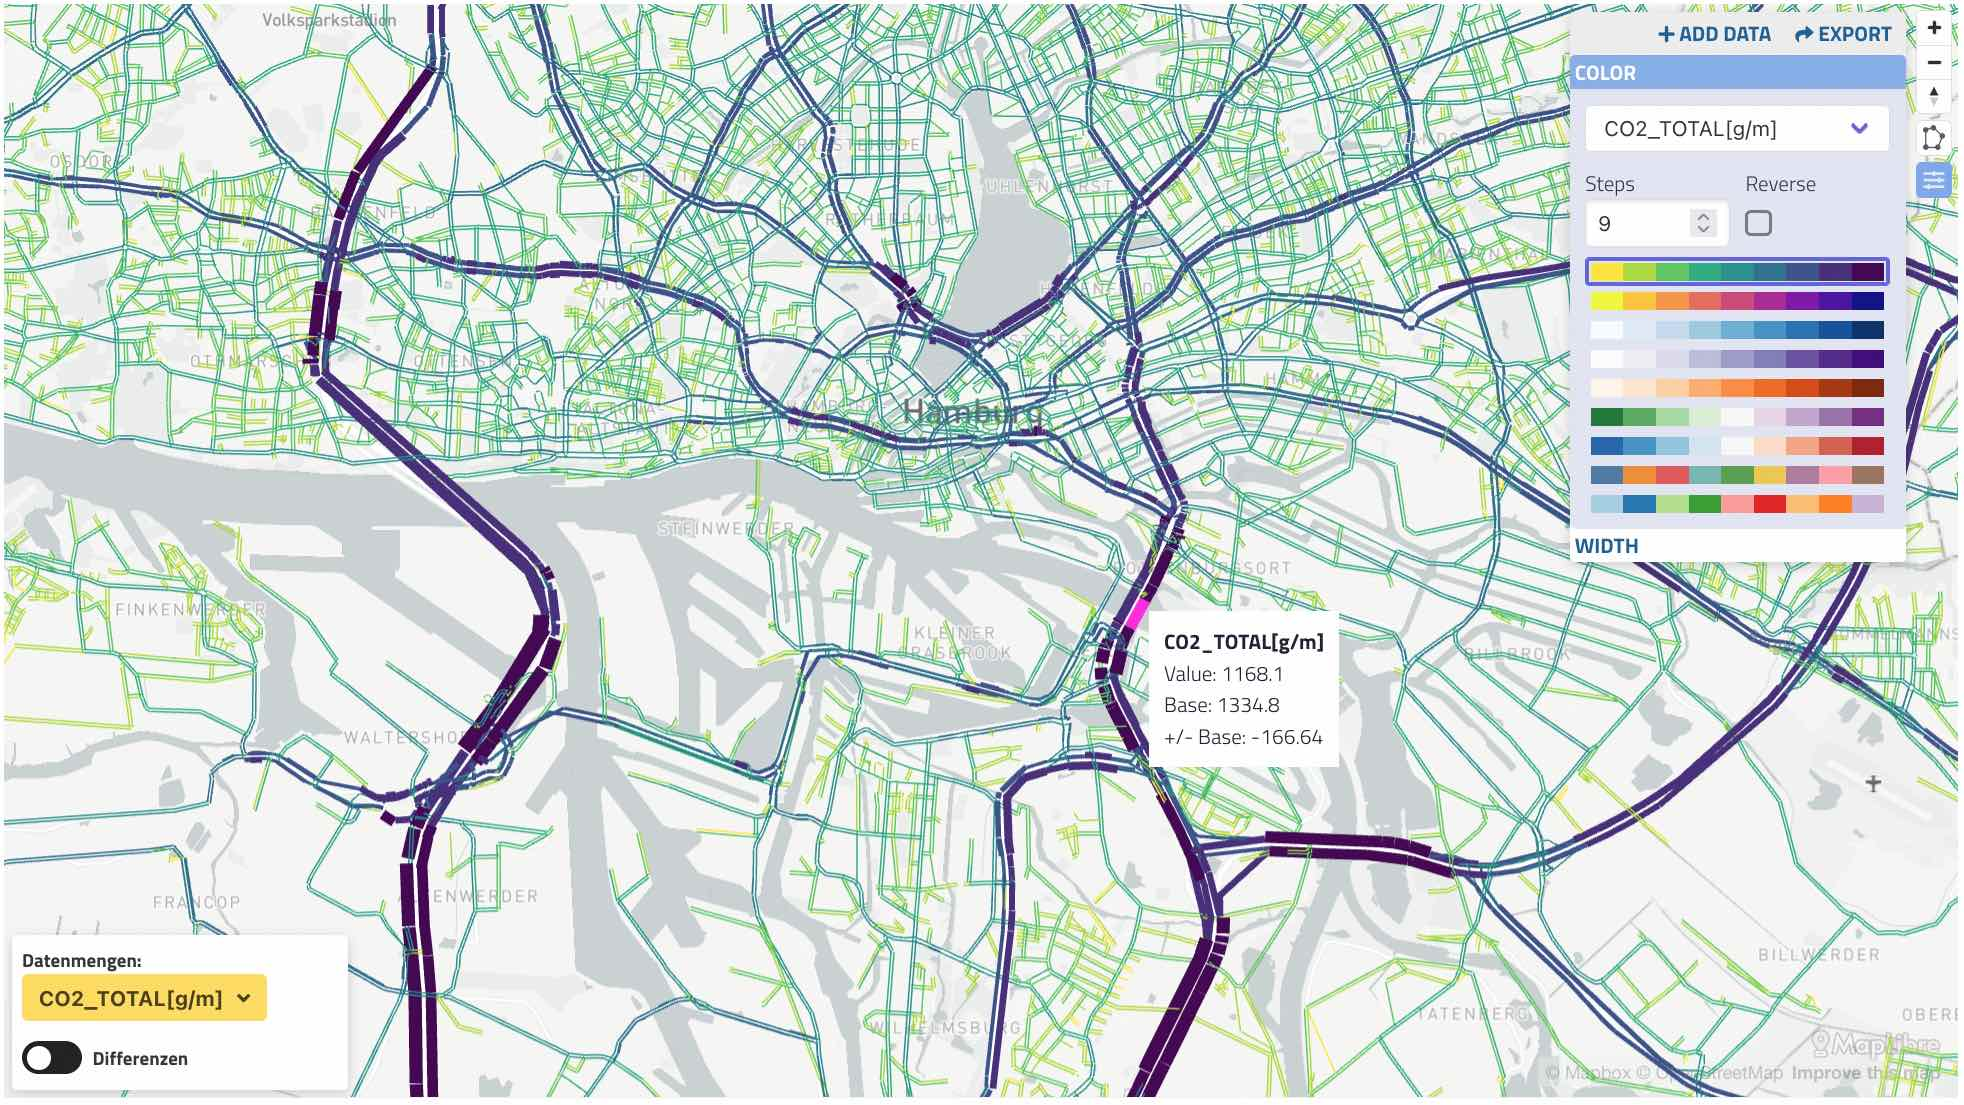
\includegraphics[width=0.8\textwidth]{assets/links.jpg}
  \caption{Bandwidth plot. Colors and widths can specify different data,}
\end{figure}

The network link plot supports typical transport ``bandwidth plots'' as
well as many other types of data. If your data can be attached to link
via the link ID, you can use this plot!

Supports display of data from multiple datasets, including ``difference
plots'' which can compare two datasets, e.g.~base vs.~build.

\hypertarget{usage}{%
\subsection{Usage}}

You can create a link visualization as a standalone view, as part of a
dashboard, or you can create it interactively from a raw network file.

\begin{enumerate}
\def\labelenumi{\arabic{enumi}.}
\item
  A standalone visualization is defined with a file named
  \texttt{viz-links-*.yaml} in your working folder. Each yaml file
  matching that pattern will produce a separate link volume diagram.
\item
  Link plots can be included in \url{dashboards} using
  \texttt{type:\ links}. See the example YAML config below.
\item
  Or, you can open a network file directly by browsing to it from the
  SimWrapper site, and then click \textbf{Add Data} in the configuration
  panel in the upper right to attache CSV data files to it. Once you
  have added data and configured the colors and widths, use the
  \textbf{Export} button to download the YAML file. Your browser will
  probably place the file in your Downloads folder; you'll need to move
  it to your data folder name it appropriately.
\end{enumerate}

\textbf{Standalone: viz-links-example.yaml}

\begin{lstlisting}
  title: 'Passagiers in DRT Vehicles'
  description: 'Hourly passengers, build scenario'
  csvFile: 'hourlyTrafficVolume-drt-vehicles.csv'
  csvBase: '../base/hourlyTrafficVolume-drt-vehicles.csv'
  network: '*output_network.xml.gz'
  thumbnail: thumbnail-roads.jpg
\end{lstlisting}

\begin{lstlisting}
  header:
  title: My Dashboard

layout:
  row1:
    - title: 'Link example'
      description: 'Sample data'
      type: links
      height: 8
      props:
        network: '../input/baseCase/hamburg-v2.0-network-with-pt-hvvArea.geo.json.gz'
        projection: EPSG:25832
        center: 13.4684, 56.6787
        zoom: 9
        showDifferences: true
        datasets:
          csvFile: 'output/reallab2030/accidentCosts.csv.gz'
          csvBase: '../base/output/accidentCosts.csv.gz'
        display:
          color:
            dataset: csvFile
            columnName: 18:00-20:00_Costs[EUR]
            colorRamp:
              ramp: Viridis
              steps: 9
          width:
            dataset: csvFile
            columnName: CostsperYear[EUR]
            scaleFactor: 100
\end{lstlisting}
\textbf{Dashboard: dashboard-example.yaml}

\hypertarget{attaching-csv-data-to-your-network-link-visualization}{%
\subsection{Attaching CSV data to your network link
visualization}\label{attaching-csv-data-to-your-network-link-visualization}}

Any CSV datafile can be used to attach data to the network
visualization. Each link in your network must have a unique ID, and the
CSV file must have one row per link, with the link ID as the first
column. No other arrangement will work.

Use whatever method you like to produce a CSV for your data; most of us
either build the dataset from event listeners within MATSim, or through
post-processing using Python or R. But as long as you can create a CSV
file with link IDs and values that you need, the method doesn't matter.

\textbf{Column names} The CSV file should have a header line as the
first line of the file. This header should contain column names, or
labels, for every column. E.g. hour of the day, type of pollutant, etc.

\begin{itemize}
\tightlist
\item
  First column \textbf{must be} the link ID, identical to the link IDs
  in the network file
\item
  All remaining columns will be available and will be labeled according
  to the file header.
\item
  \textbf{Note:} older versions of SimWrapper used to autogenerate a
  ``sum'' column. This has been removed. If you want to show a ``sum''
  total column, you will have to calculate it yourself as a separate
  column in your data file.
\end{itemize}

\begin{center}\rule{0.5\linewidth}{0.5pt}\end{center}

\hypertarget{yaml-fields-explained}{%
\subsection{YAML fields explained}}

*Filename fields** can refer to subfolders and to parent folders using
\texttt{"../"}.

\begin{itemize}
\tightlist
\item
  example: \texttt{network:\ :\ "../networks/base.json.gz"}
\end{itemize}

This works as far up the hierarchy as the base of the filesystem,
specified in \texttt{fileConfig.js} but no further.

\hypertarget{field-descriptions}{%
\subsubsection{Field descriptions}\label{field-descriptions}}

\textbf{title:} (optional) title of the visualization, appears right on
top of the map. If a title is specified both under \texttt{general} and
under \texttt{props}, the one under \texttt{general} will be used.

\noindent\textbf{description:} (optional) description of the visualization,
appears between title and map. If a description is specified both under
\texttt{general} and under \texttt{props}, the one under
\texttt{general} will be used.

\noindent\textbf{csvFile:} dataset in CSV or TSV format.

\begin{itemize}
\tightlist
\item
  Columns are autodetected and will split at commas, semicolons, or
  tabs.
\item
  Numbers \textbf{must be in 1234.56 format} -- European
  ``1.234.567,00'' formats will not work.
\end{itemize}

\noindent\textbf{csvBase:} (optional) ``base'' dataset for difference plots. If
\texttt{csvBase} is specified, ``diff mode'' will be enabled and
difference plots can be automatically generated.

\begin{itemize}
\tightlist
\item
  Differences are always calculated as
  \texttt{\textquotesingle{}csvFile\ -\ csvBase\textquotesingle{}}
\end{itemize}

\noindent\textbf{network:} Specify either at MATSim
\texttt{output\_network.xml.gz} network file, or a geojson-format
network file. The geojson format loads much faster, but requires that
you create it first.

\begin{itemize}
\tightlist
\item
  Use the python script
  \href{https://raw.githubusercontent.com/simwrapper/simwrapper/master/scripts/create-geojson-network.py}{create-geojson-network.py}
  to create a geojson network from a MATSim network.xml.gz file.
\item
  Command is
  \texttt{python\ create-geojson-network.py\ {[}my\_output\_network.xml.gz{]}\ {[}Projection{]}}
\item
  and will create a file with the name \texttt{mynetwork.geo.json.gz}.
\end{itemize}

\noindent\textbf{projection:} projection must be given! Format
\texttt{EPSG:25832} etc.

\noindent\textbf{geojsonFile:} (deprecated) - same as \texttt{network}.

\noindent\textbf{thumbnail:} (optional) file path to a thumbnail in jpg format

\noindent\textbf{center:} (optional) coordinates that the map centers on. Can be
provided as array or string. If it is not provided, a center is
calculated using a sampling of the data.

\noindent\textbf{zoom:} (optional) zoom level of the map. If it is not provided,
the zoom level 9 is used.

\noindent\textbf{showDifference:} allows difference plots to be created if a base
case is provided. Should be \texttt{true}.

\noindent\textbf{display:} The optional display section includes details of the
color and width data specifications.

\hypertarget{defining-colors-and-widths}{%
\subsection{Defining Colors and
Widths}\label{defining-colors-and-widths}}

Both colors and widths can be based on the CSV data. They are defined in
the \texttt{display:} section of the YAML; see the example above.

\hypertarget{color}{%
\subsubsection{Color}\label{color}}

The \texttt{color} section may include the following properties:

\begin{itemize}
\tightlist
\item
  \textbf{dataset} required. The ID of the csv datafile itself; in the
  example above, \texttt{csvFile} is one key and \texttt{csvBase} is
  another. This tells SimWrapper which dataset you want to use.
\item
  \textbf{columnName} The name of the column containing color values
\item
  \textbf{colorRamp} This section can have multiple settings:

  \begin{itemize}
  \tightlist
  \item
    \texttt{ramp}: The name of the color progression; can be
    \texttt{Viridis}, \texttt{Plasma}, \texttt{Blues}, \texttt{Purples},
    \texttt{Oranges}, \texttt{PRGn}, \texttt{RdBu}, \texttt{Tableau10},
    \texttt{Paired}. Note that \texttt{PRGn} and \texttt{RdBu} are
    \textbf{diverging scales}, while \texttt{Tableau10} and
    \texttt{Paired} are appropriate for \textbf{categorical} instead of
    sequential data.
  \item
    \texttt{reversed} true or false, flips the order of colors
  \item
    \texttt{steps} the number of different colors in the progression;
    default is 9.
  \end{itemize}
\end{itemize}

\hypertarget{width}{%
\subsubsection{Width}\label{width}}

The \texttt{width} section includes the following properties:

\begin{itemize}
\tightlist
\item
  \textbf{dataset} required. The ID of the csv datafile itself; in the
  example above, \texttt{csvFile} is one key and \texttt{csvBase} is
  another. This tells SimWrapper which dataset you want to use.
\item
  \textbf{columnName} The name of the column containing width values
\item
  \textbf{scaleFactor} Values will be \textbf{divided by} this scaling
  factor. Set this to \texttt{0} to have constant, paper-thin widths.
\end{itemize}

\paragraph{example-data.csv} Sample CSV data

\begin{verbatim}
link;01:00:00;02:00:00;03:00:00;04:00:00;05:00:00;06:00:00;00;00
72539930;0;0;0;0;7;13;20;16;13;15;18;17;32;25;29;55;53;43;48;12;12;
42868713;0;0;0;0;0;0;0;0;0;0;0;0;0;1;0;0;1;1;0;0;0;0;0;0;0;0;0;0;0
72539936;0;1;0;0;17;57;63;52;51;47;49;59;78;67;73;113;99;98;107;47;
6173553;0;1;0;3;5;1;10;10;9;3;8;4;6;3;4;9;5;7;4;2;1;1;1;2;0;1;0;0;0
\end{verbatim}

\hypertarget{deprecated-fields-do-not-use}{%
\subsection{Deprecated fields, do not
use:}\label{deprecated-fields-do-not-use}}

\textbf{shpFile,dbfFile, shpFileIdProperty:} (deprecated) filenames for
the alternative, slower network file in shapefile format. Don't use this
if you have created the geojson network file above.

\noindent\textbf{widthFactor:} (deprecated) Width values used to be uniformly
scaled by this value.

\noindent\textbf{sampleRate:} (deprecated) This option used to specify the MATSim
simulation sample rate; i.e.~a 1\% sample would use \texttt{0.01} here
so that volumes were scaled properly. This is NOW IGNORED; you must
scale your CSV data appropriately.
